\documentclass[a4paper,man,natbib,donotrepeattitle, apacite]{apa6}
\usepackage{authblk}% for multiple authors
\usepackage{tabularx} % to create tables in methods

\usepackage[english]{babel}
\usepackage[utf8x]{inputenc}
\usepackage{amsmath}
\usepackage{graphicx}
\usepackage[colorinlistoftodos]{todonotes}
\geometry{reset, letterpaper, height=9in, width=7in, hmarginratio=1:1, vmarginratio=1:1, marginparsep=0pt, marginparwidth=0pt, headheight=15pt}
\usepackage{tikz}
\usepackage{wrapfig}
\usepackage{amssymb}
\usepackage{amsmath,subcaption,caption}
\usepackage{ifxetex,ifluatex}
\usepackage{fixltx2e,authblk} % provides \textsubscript
\usepackage{lmodern}
\usepackage[T1]{tipa}
\usepackage{longtable,booktabs}


\title{\LARGE Practice and experience predict coarticulation in child speech}

\shorttitle{Coarticulation in child speech}

\usetikzlibrary{shapes.geometric, arrows,backgrounds,fit,positioning}

\author[1,2]{\large Margaret Cychosz}
\author[1]{Jan R. Edwards}
\author[3]{Benjamin Munson}

\affil[1]{\small Department of Hearing and Speech Sciences, University of Maryland, College Park}
\affil[2]{Center for Comparative and Evolutionary Biology of Hearing, University of Maryland, College Park}
\affil[3]{Department of Speech-Language-Hearing Sciences, University of Minnesota, Twin Cities}

\affiliation{} % to remove weird affiliation

\clearpage
\authornote{Author to whom correspondence should be addressed: Margaret Cychosz, 0100 Samuel J. LeFrak Hall, University of Maryland, College Park, College Park, USA, 20742. Email: mcychosz@umd.edu.}






\abstract{Much research in child speech development suggests that young children coarticulate more than adults. There are two possible, not mutually-exclusive, explanations for this pattern. First, children may coarticulate more as a performance error, because they are limited by immature motor control. Children might also coarticulate more because they initially represent phonological segments in larger, more holistic units such as syllables or feet. We tested these explanations by measuring four-year-old children’s coarticulation between adjacent segments in real words and paired nonwords. Children coarticulated significantly less between the same sound sequences in real words than nonwords. Children with larger vocabularies also coarticulated less, especially in real words. Finally, for children who had completed daylong audio recordings, we found that children who vocalized more throughout the day coarticulated less. Quantity of child vocalizations was more predictive than a measure of receptive language experience, adult word count, suggesting a strong role of self-practice for the development of coarticulation.}

\keywords{speech development, speech production, coarticulation, phonology, word repetition, naturalistic recording}


\begin{document}
\setlength\parindent{24pt} % indent each paragraph



\maketitle

\setcounter{secnumdepth}{2} % number sections

\section{Introduction}

A long standing question in language development is whether the representation of linguistic forms differs between adults and children. Numerous experimental paradigms and techniques examining speech perception and lexical access (e.g. head-turn preference, eye-tracking), have addressed this question \cite{majoranoRelationshipInfantsProduction2014, storkelLexiconPhonologyInteractions2002,swingleyLexicalNeighborhoodsWordForm2002}. However, increasingly, children’s own speech production has been studied to shed light on the nature of their phonological representations \cite{fergusonWordsSoundsEarly1975,goffmanBreadthCoarticulatoryUnits2008,nittrouerEmergencePhoneticSegments1989,nittrouerHowChildrenLearn1996,noiraySpokenLanguageDevelopment2019,noirayHowChildrenOrganize2018,redfordGrammaticalWordProduction2018,songEffectsCoarticulationMorphological2013,songDurationalCuesFricative2013,zharkovaCoarticulationIndicatorSpeech2011}. These works have demonstrated that speech production patterns, such as the duration, variability, and especially fluency of speech, can lend insight into speakers’ phonological representations and planning. 

One production metric that is frequently used to measure speech fluency in development is coarticulation, or the temporal and gestural overlap that results from producing two speech sounds in a sequence \cite{gerosaAnalyzingChildrenSpeech2006,goffmanBreadthCoarticulatoryUnits2008,zharkovaCoarticulationIndicatorSpeech2011}. Coarticulation is not simply noise in the speech signal. It conveys important auditory-acoustic information for speakers and listeners alike. Appropriate coarticulatory overlap, such as the ability to anticipate forthcoming speech segments, indicates mature, adult-like speech \cite{barbierWhatAnticipatoryCoarticulation2020,bradlowConfluentTalkerListeneroriented2002,whalenCoarticulationLargelyPlanned1990}. Children speak more slowly overall, and with less coordinated movement \cite{greenPhysiologicDevelopmentSpeech2000,goffmanRelationsSegmentalMotor2007,leeAcousticsChildrenSpeech1999}. It might then be logical to conclude that children coarticulate less than adults. Support for this notion comes from some studies finding that children show less long-distance anticipatory coarticulation, for example across syllable boundaries (\citeNP{barbierWhatAnticipatoryCoarticulation2020}; cf. \citeNP{goffmanBreadthCoarticulatoryUnits2008}; \citeNP{rubertusDevelopmentGesturalOrganization2018,rubertusVocalicActivationWidth2020}). Within syllables or between adjacent segments, however, a large number of studies now suggest that children coarticulate more than adults \cite{nittrouerHowChildrenLearn1996,noirayBackFutureNonlinear2019,zharkovaSpatialTemporalLingual2014}. It is thought that children may eventually engage in less anticipatory coarticulation as they age because they have more experience, and practice, with language and speech production. 

\subsection{The development of coarticulation}

Traditionally, there have been two not mutually-exclusive explanations for why children coarticulate between adjacent segments more than adults. Children’s coarticulation could reflect 1) performance errors due to the development of fine motor control and 2) the phonological reorganization of speech from more holistic units, such as syllables, into phonemes. 

First, children could coarticulate more because their fine motor control develops gradually throughout childhood and well into early adolescence \cite{barbierWhatAnticipatoryCoarticulation2020,kentAnatomicalNeuromuscularMaturation1976,perkellFiveDecadesResearch2013,walshArticulatoryMovementsAdolescents2002}. The spatiotemporal coordination of the lips and jaw, for example, undergoes significant development between ages two and six---younger children tend to rely more on vertical jaw movement, only learning to simultaneously coordinate both the lips and jaw with age \cite{greenPhysiologicDevelopmentSpeech2000}. Unsurprisingly, this motor control development has implications for children’s phonetic production, including coarticulation. For example, \citeauthor{zharkovaDynamicsVoicelessSibilant2018} (2018) measured coarticulation within /\textschwa sV/ and /\textschwa \textesh V/ sequences in children aged 7;0-13;0 and adults and found both that the ability to differentiate between /s/ and /\textesh/ increased with age and that the youngest children were most variable. The authors attribute these findings to the children’s developing control of the tongue, especially its coordination with the lips and jaw. \citeauthor{rubertusDevelopmentGesturalOrganization2018}(2018) likewise attribute 3;6-7;0 children’s coarticulation patterns---all children engaged in more V-V anticipatory coarticulation than adults---to protracted lingual coordination.           

Another reason younger children might coarticulate more than adults and older children is because they initially represent language more holistically than adults, in units such as syllables, feet, or morae, instead of phoneme-sized segments. These larger units would then be activated during children’s speech planning resulting in significant anticipatory effects of adjacent segments on one another. Anticipatory coarticulation between adjacent phones then decreases with age\footnote{The literature remains somewhat mixed on the directionality of coarticulatory development. Some studies have been unable to find a difference between adult and child coarticulation between adjacent segments \cite{katzAnticipatoryCoarticulationSpeech1991,noirayDevelopmentMotorSynergies2013,serenoDevelopmentalAspectsLingual1987,zharkovaDynamicsVoicelessSibilant2018}, while others have found that children coarticulate less \cite{kentSegmentalOrganizationSpeech1983}.} as phonological units reorganize into smaller segments in a process often termed phonological reorganization \cite{goodellAcousticEvidenceDevelopment1992,nittrouerEmergencePhoneticSegments1989,nittrouerHowChildrenLearn1996,noiraySpokenLanguageDevelopment2019,noirayHowChildrenOrganize2018,redfordGrammaticalWordProduction2018,zharkovaCoarticulationIndicatorSpeech2011}.\footnote{It is important to underscore how this phonological reorganization could play out differently cross-linguistically. Results from tests of phonological awareness in Mandarin-speaking children, for example, suggest that syllable and tone awareness are more important for character recognition than sub-syllabic awareness (McBride-Chang et al., 2004; Shu et al., 2008). The developmental trajectories of phonological reorganization may then differ based on the language of exposure.}  

There is no doubt that fine motor control develops with age, with clear implications for children’s speech faculty and coarticulation \cite{barbierWhatAnticipatoryCoarticulation2020,zharkovaDynamicsVoicelessSibilant2018}. However, there is also ample evidence suggesting that child coarticulation is explained by phonological reorganization. Support for this idea often comes from studies with cross-sectional designs: numerous studies, measuring coarticulation between the same segments using the same methods (e.g. acoustics, articulatory), have shown that children coarticulate less between adjacent segments as they age. 
In a series of studies, \citeauthor{nittrouerEmergencePhoneticSegments1989} (1989) and \citeauthor{nittrouerHowChildrenLearn1996} (1996) found that as children aged 3;0-8;0 got older, they tended to coarticulate less between segments in fricative-vowel sequences. Similar conclusions were drawn by \citeauthor{zharkovaCoarticulationIndicatorSpeech2011} (2011) who measured children’s (aged 6;0-9;0) coarticulation using articulatory imaging methods (ultrasound) and found that the degree of coarticulation decreased with age. Finally, in a cross-sectional sample of children aged 3;6-7;0, \citeauthor{noirayHowChildrenOrganize2018} (2018) also found that children coarticulated less in CVC sequences as they aged. However, the authors warn that this may not be attributable to a single representational strategy, such as the representation of speech in syllables or chunks. Rather, there may be different organizational---and thus production---strategies for different segments. Children must learn the degree of coarticulation permitted between phones in sequences such as /bi/ as opposed to that permitted in /di/ or /gi/. (See also Zharkova [2018] for discussion of segment-specific effects on coarticulation.) 

The aforementioned studies used a cross-sectional study design to support the idea that children’s coarticulatory patterns reflect phonological reorganization. However, cross-sectional designs cannot rule out the exclusive role of speech motor control for coarticulatory development because motor control coincides with phonological reorganization over the course of development---both develop and change as children age. As a result, the underlying causes behind children’s coarticulatory patterns have somewhat eluded researchers because many common methodological designs have not attempted to decouple the motor maturation and phonological reorganization explanations (cf. \citeNP{noiraySpokenLanguageDevelopment2019}).

Additional evidence in support of phonological reorganization needs to come from predictors that, unlike age, develop relatively independently of speech motor control. \citeauthor{noiraySpokenLanguageDevelopment2019} (2019) correlated children’s coarticulation with two such independent measures of linguistic experience---vocabulary size and phonological awareness (i.e. metalinguistic recognition of phoneme-sized units). Neither of these factors should depend greatly upon motor maturation. The authors found that children (aged 4;0-7;0)  with greater phonological awareness, and larger expressive vocabularies, coarticulated less between segments, independent of chronological age. From these findings the authors conclude that children’s coarticulation is likely explained by both speech motor control maturation and phonological reorganization. 

To be clear, the motor maturation and phonological reorganization explanations for children’s coarticulation are not mutually exclusive. Children’s fine motor planning is continuously honed and developed as children age, with implications for child coarticulation---these conclusions are clear \cite{barbierWhatAnticipatoryCoarticulation2020,rubertusDevelopmentGesturalOrganization2018,zharkovaDynamicsVoicelessSibilant2018}. The objective of the present analysis is to determine to what extent children’s speech representations also explain their coarticulatory patterns, over and above the role of fine motor development. To do so, the current study expands upon \citeauthor{noiraySpokenLanguageDevelopment2019} (2019) by evaluating the role of several additional independent factors on child coarticulation: speech planning, vocabulary size, and the language environment. In typically-developing children, these factors should develop relatively independent of speech motor control. Consequently, if one or more of them predicts the degree of children’s coarticulation, it suggests influences beyond motor control for the development of coarticulation, shedding further light on the underlying causes of coarticulation in development. 

First, the current study evaluates the role of speech planning on children’s coarticulation by measuring coarticulation between CV sequences embedded in nonwords and matched real words (e.g. [su] in the nonword \textit{sudras} versus the real word \textit{suitcase}). Unlike real words, nonwords must be produced without the support of lexical, semantic, or complete phonetic representations \cite{chiatPreschoolRepetitionTest2007,cychoszLexicalAdvantageFouryearold2020,gathercoleInfluencesNumberSyllables1991,keren-portnoyRoleVocalPractice2010}. Consequently, nonwords place additional demands upon children during speech planning which could result in less fluent production, or less coarticulation.

Second, in an attempt to replicate \citeauthor{noiraySpokenLanguageDevelopment2019} (2019), this study evaluates the role of vocabulary size on coarticulation---though we expand upon \citeauthor{noiraySpokenLanguageDevelopment2019} (2019) by comparing the role of receptive and expressive vocabularies. Vocabulary size could be expected to predict coarticulation because it predicts the emergence of discrete phonological units during development \cite{edwardsInteractionVocabularySize2004,sosaLexicalPhonologicalEffects2012,stoel-gammonRelationshipsLexicalPhonological2011,storkelLexiconPhonologyInteractions2002} and, most relevant for the current work, speech accuracy and fluency \cite{cychoszLexicalAdvantageFouryearold2020,edwardsInteractionVocabularySize2004,metsalaYoungChildrenPhonological1999,munsonRelationshipsNonwordRepetition2005,zamunerPhonotacticProbabilitiesOnset2009}. Children with larger receptive vocabularies have more unique word types over which they can generalize to infer the importance of certain segments in their native language(s). Those with larger expressive vocabularies also have more practice producing more unique words, and thus phoneme combinations, potentially resulting in further segmental production mastery \cite{beckmanGeneralizingLexiconsPredict2010}. For these reasons, both expressive and receptive vocabulary sizes are expected to predict degree of coarticulation in children. 

The third predictive factor for coarticulation evaluated here is the language environment. This is measured by correlating elements from children’s daily language environments---namely the frequency of child vocalizations---with coarticulation. The language learning environment has been shown to predict a number of developmental milestones in speech and language including lexical processing \cite{weislederTalkingChildrenMatters2013}, expressive and receptive vocabulary sizes \cite{hartMeaningfulDifferencesEveryday1995,hoffSpecificityEnvironmentalInfluence2003,mahrUsingLanguageInput2018}, and babbling complexity \cite{ferjanramirezParentCoaching102019}. It is thus reasonable to predict that children’s daily linguistic experiences, specifically how frequently they vocalize, could likewise predict their coarticulation patterns. 

The factors of speech planning, vocabulary size, and the language environment all concern the role of speech production practice for coarticulatory development. For example, we anticipate that real words will be produced more fluently than nonwords in part because children have more practice producing the real words. A similar argument can be made for the potential roles of expressive vocabulary size and vocalization frequency on child coarticulation. The following section outlines why speech production practice may be expected to predict children’s coarticulation patterns. 

\subsection{The role of production practice for phonological development}

A child’s developing anatomy is highly transient with anatomical changes that are non-linear \cite{vorperianDevelopmentVocalTract2005} and non-uniform because different speech articulators mature at distinct rates \cite{nittrouerEmergenceMatureGestural1993}. These elements of phonological development present a challenge for children who must establish accurate, replicable, articulatory-acoustic mappings in the face of rapid, uneven anatomical change. It is analogous to shooting an arrow at a bullseye with an ever-changing ratio of arm to bow length. 

The lack of established articulatory routines in children has repercussions for their phonological representations. While speech perception and perceptual narrowing mechanisms in infancy are vital to establish phonological representations for a child’s native language, some evidence suggests that articulation and production practice may also play a role \cite{brudererSensorimotorInfluencesSpeech2015,keren-portnoyRoleVocalPractice2010,mcallisterbyunMotorInfluencesGrammar2016,mennChallengesTheoriesCharges2013,vihmanLearningWordsLearning2017,zamunerReverseProductionEffect2018}. Phonological representations then consist of abstract phonological categories and accompanying articulatory routines. For very young children’s speech, an ``articulatory filter'' has been cited to formalize this notion \cite{depaolisProductionPatternsInfluence2011,depaolisInfluenceBabblingPatterns2013,laingBabbleWordsInfants2020,vihmanVariablePathsEarly1993,vihmanLearningWordsLearning2017}. According to this theory, when a child hears a sound in their ambient language, that sound may become more salient and recognizable, causing the child to produce it more. Consequently, representations that encode articulatory information may be in place even before infants reliably produce word forms \cite{brudererSensorimotorInfluencesSpeech2015}. 

There is ample evidence for a production effect, or strengthened phonological representations that ensue from production practice. \citeauthor{depaolisProductionPatternsInfluence2011} (2011) tested infants aged 0;10-1;4 on preference for ``own production'' consonants (consonants that the infant was already producing consistently) versus ``other production'' consonants (consonants that the infant was not yet producing consistently). In a head-turn preference task, the authors found that those infants who were already producing multiple consonants paid more attention to the ``other production'' consonants. At the same time, there was no effect for infants who were producing one or no consonants at the time of testing. The authors suggest that, in conjunction with early speech perception, the infants’ preference for novel consonants may strengthen early speech acquisition. For one thing, these novel sounds may become more salient for an infant in the input. A resultant ``auditory feedback loop'' \cite{majoranoRelationshipInfantsProduction2014} could facilitate phonological development as children’s articulatory practice coincides with acoustic-auditory speech representations (see \citeauthor{depaolisInfluenceBabblingPatterns2013} [2013] \& \citeauthor{keren-portnoyRoleVocalPractice2010} [2010] for similar conclusions). 

In older children, production practice in the form of repeating whole words could also be advantageous for phonological development (\citeNP{ichtProductionEffectMemory2015,mcallisterbyunAmapModelArticulatory2016,mcallisterbyunMotorInfluencesGrammar2016}; cf. \citeNP{zamunerReverseProductionEffect2018}. The argument behind this production effect in older children is that by producing a word, children are better able to encode the word’s auditory-acoustic signature in semantic and phonological representations. The time required to process a new word may decrease if the word contains a well-practiced motor scheme, for example a phonotactically-probable sequence, learned elsewhere \cite{storkelComparisonHomonymNovel2005,storkelInfluencePartwordPhonotactic2011}. \citeauthor{ichtProductionEffectMemory2015} (2015) found that 5-year-old children remembered novel words better when they looked at a picture of a novel object and produced the new word out loud than when they looked at the object and only heard the experimenter repeat the item name. Most recently, however, \citeauthor{zamunerReverseProductionEffect2018} (2018) found that 4;5-6;0 children remembered novel words better during a ``hear only'' condition than a ``hear and produce'' condition, suggesting that the production effect may vary by task demand and the child’s developmental stage. 

A final way that the production effect could affect phonological development is through parental engagement. Infants and children, of various ages, who produce more speech tend to elicit more parental responses \cite{franklinEffectsParentalInteraction2014,goldsteinSocialFeedbackInfants2008,mcgillionWhatPavesWay2017,pretzerInfantadultVocalInteraction2019,warlaumontSocialFeedbackLoop2014}. Positive correlations have been found between the number of words spoken by adults in the environment and the frequency of children’s own vocal productions for children aged 0;2-4;0 \cite{gilkersonImpactAdultTalk2009,orenaReliabilityLanguageEnvironment2019,weislederTalkingChildrenMatters2013}. \citeauthor{franklinEffectsParentalInteraction2014} (2014) and \citeauthor{goldsteinSocialFeedbackInfants2008} (2008) illustrate how this engagement effect plays out for infant vocalizations. \citeauthor{franklinEffectsParentalInteraction2014} (2014) demonstrated that infants who were presented with a still face after interacting with parents vocalized more to re-engage parents. And \citeauthor{goldsteinSocialFeedbackInfants2008} (2008) found that infants (aged 0;9) adapted the structure of their babble shapes (i.e. proportion of CV syllables) to match caregiver productions, but only when the caregivers spoke contingently to the infants by, for example, moving closer to, smiling at, or touching the infant. Thus, children’s vocalizations engage parents \cite{albertSocialFunctionsBabbling2018}, whose responses, in turn, encourage infants to vocalize more. 

To summarize, speech production and practice appear to predict phonological development. This production effect starts early, as infants engage in social feedback loops with caregivers that result in increased infant vocal exploration and practice \cite{franklinEffectsParentalInteraction2014,goldsteinSocialFeedbackInfants2008,mcgillionWhatPavesWay2017,pretzerInfantadultVocalInteraction2019,warlaumontSocialFeedbackLoop2014}. Parental input is still correlated with the frequency of children’s vocalizations into toddlerhood 
\cite{gilkersonImpactAdultTalk2009,weislederTalkingChildrenMatters2013}. The practice effect also manifests in infants and young toddlers who, during vocal exploration and late babbling stages, produce those sounds that are most salient and frequent in their environments \cite{depaolisProductionPatternsInfluence2011,depaolisInfluenceBabblingPatterns2013,laingBabbleWordsInfants2020,vihmanVariablePathsEarly1993,vihmanLearningWordsLearning2017}. Finally, speech practice also appears to facilitate lexical acquisition, with ramifications for phonological development \cite{sosaLexicalPhonologicalEffects2012,stoel-gammonRelationshipsLexicalPhonological2011,zamunerPhonotacticProbabilitiesOnset2009}: there may be an advantageous effect of production whereby children learn new words faster by articulating them than hearing alone (\citeNP{ichtProductionEffectMemory2015}; but cf. \citeNP{zamunerReverseProductionEffect2018}). The strong predictive role of practice leads us to make several predictions for the factors studied in the current work, which are outlined below. 

\section{The current study}

The goal of the present study is to study the role of three factors that could potentially underlie children’s coarticulatory patterns in spoken language: speech planning, vocabulary size (expressive and receptive), and the language environment. Again, the tendency for children to coarticulate is almost certainly due, in part, to their overall inexperience with speech production and immature speech motor control development \cite{barbierWhatAnticipatoryCoarticulation2020,goffmanRelationsSegmentalMotor2007,greenPhysiologicDevelopmentSpeech2000,rubertusDevelopmentGesturalOrganization2018,zharkovaDynamicsVoicelessSibilant2018}. Here we are interested in the potential contribution of factors that may develop independently of fine motor development. 

To test how speech organization may contribute to children’s coarticulation, we examined four-year-old children’s spoken language production in nonwords and corresponding real words. Each real word had a paired, word-initial CV syllable in the nonword (e.g. [su] in \textit{sudras} and \textit{suitcase}). This lexicality condition allowed us to test how both speech and lexical planning contribute to children’s tendency to coarticulate. The children have experience hearing and, crucially, producing, the real words but not the nonwords. How will children’s existing lexical representations and articulatory schemata affect their spoken coarticulation patterns? We made the following prediction concerning child coarticulation in real words and paired nonwords:

\begin{enumerate}
\item[1.] Because children already have experience producing the real words, they will coarticulate less within CV sequences when they are embedded in real words (e.g. \textit{suitcase}) than nonwords (e.g. \textit{sudras}).\footnote{Hypotheses one and two were originally pre-registered to predict that 1) children would coarticulate more in real words than nonwords and 2) that children with larger vocabularies would coarticulate more than children with smaller vocabularies \cite{cychoszSpectralTemporalMeasures2019}. However, these hypotheses were registered prior to the publication of \citeauthor{noiraySpokenLanguageDevelopment2019} (2019). Those authors found that greater linguistic experience---vocabulary size and phonological awareness---predicted less coarticulation. In light of those results, we eventually adjusted our hypotheses but for the sake of open science, transparency, and replicability, we acknowledge that our original hypotheses actually predicted the reverse.}

\end{enumerate}

We then correlated the children’s spoken language patterns with their vocabulary size (receptive and expressive) and elements from each child’s naturalistic language environment (measured with daylong audio recordings). We made two predictions concerning these factors:

\begin{enumerate}
\item[2.] \citeauthor{noiraySpokenLanguageDevelopment2019} (2019) found that children with larger expressive vocabularies coarticulated less. As a result, we predict that children who have larger lexicons, estimated as the size of their expressive or receptive vocabularies, will coarticulate less between the segments in CV sequences. We build on the work of \citeauthor{noiraySpokenLanguageDevelopment2019} (2019) by comparing the roles of expressive and receptive vocabulary sizes for coarticulation, though we do not make a specific prediction for which measure of vocabulary size will be the stronger predictor.

\item[3.] Children who produce more language, quantified as the frequency of child vocalizations during daylong audio recordings, will coarticulate less between segments in CV sequences.
\end{enumerate}

\section{Methods}

\subsection{Participants}

One hundred and three children (56 girls, 47 boys) aged 3;3 to 4;4 (years;months, mean=3;5, SD=0;3) participated in the study. All children were monolingual speakers of English participating in a longitudinal study studying children’s phonological development. The current data were collected on the second of the child’s three scheduled visits, approximately one year after the first visit. All families consented to participate in the research upon their initial visit to the lab. All in-lab tasks were completed at the University of Wisconsin, Madison or the University of Minnesota, Twin Cities. 

Each participant passed a hearing screening in at least one ear at 25dB for 1000, 2000, and 4000Hz. Per parental self-report, 90 (87.4\%) of the children had normal speech and hearing development. The 13 remaining children were identified as late talkers by their caregivers. It should be noted that this was a caregiver description, rather than a clinical diagnosis. The caregiver-identified late talkers and caregiver-identified typically-developing children are differentiated in the Results and in statistical modeling. 

Socioeconomic status, quantified as mother’s education level, was reported by caregivers. 38\% of mothers had a graduate degree, 32\% a college degree, 21\% some college/trade school/associate degree, 7\% a high school diploma, and 2\% did not have a high school diploma. 

\subsection{Word repetition tasks}

For the in-lab data collection phase, children completed two picture-prompted word repetition tasks: a nonword repetition task, where participants repeated nonce words after an adult model speaker, and a real word repetition task. The experiments and pre-task assessments were completed in two 1-hour test sessions on different days, usually separated by about a week. Children always completed the real word repetition task during the first testing session and the nonword repetition task during the second session. The decision was made to have the children complete the repetition tasks on separate days because real word and nonword tasks are generally given separately \cite{chiatPreschoolRepetitionTest2007}. In addition, we chose not to counterbalance the presentation order of the two word repetition tasks because in our experience conducting speech elicitation paradigms with children of this age, we have found that children sometimes perceive phonotactically-probable nonwords as real words. Furthermore, children of this age do not readily switch back and forth easily between nonwords and real words. See \citeauthor{cychoszLexicalAdvantageFouryearold2020}(2020) for further justification of the presentation order for the repetition tasks.                                          
\subsection{Repetition task materials}

The real word stimuli for the word repetition tasks were chosen from lists such as the ``Toddler Says'' portion of the MacArthur Bates Communicative Development Inventory \cite{fensonMacArthurBatesCommunicativeDevelopment2007}, to ensure familiarity to the majority of children in this age group (see Table \ref{tab:stimuli}). Real word repetition task object names were color photographs of the objects. Nonword repetition task object names were color photographs of unfamiliar tools, plants, fruit, etc. All stimuli images and sound files are available to use for replication in our Open Science Framework project (\url{https://osf.io/dcb9p/}). 


\begin{table}
\centering
\caption{\label{tab:stimuli}Stimuli used in word repetition tasks}

\begin{tabular}{c c | c c} 
\hline
\textsc{Real word} & \textsc{Nonword} & \textsc{Real word} & \textsc{Nonword} \\
\hline

\midrule

 candle {[}k\ae nd\textschwa l{]} &  `kamig' {[}k\ae m\textsci g{]} & 
 sidewalk
{[}sa\textsci dwak{]} &  `sighprote' {[}sa\textsci p\textturnr ot{]} \\

chicken {[}t\textesh \textsci k\textschwa n{]} & `chihmig' {[}t\textesh \textsci m\textsci g{]} & sister
{[}s\textsci st\textschwa \textturnr{]} &  `sihplok' {[}s\textsci plok{]} \\

 {coffee {[}kafi{]}} &  {`kahsep' {[}kas\textepsilon p{]}} &  {suitcase
{[}sutkes{]}} &  {`soodros' {[}sud\textturnr as{]}}\tabularnewline

 {cutting {[}k\textturnv t\textsci \ng{]}} &  {`kuhfeem' {[}k\textturnv fim{]}} &  {sunny
{[}s\textturnv ni{]}} &  {`suhbith' {[}s\textturnv b\textsci\texttheta{]}} \\

 {kitchen {[}k\textsci t\textesh \textschwa n{]}} &  {`kihpon' {[}k\textsci pon{]}} &  {tiger
{[}ta\textsci g\textschwa \textturnr{]}} &  {`tieblor' {[}ta\textsci blo\textturnr {]}}\tabularnewline

 {raisins {[}\textturnr ez\textsci nz{]}} &  {`raebith' {[}\textturnr eb\textsci\texttheta{]}} &  {toaster
{[}tost\textschwa \textturnr{]}} &  {`toezell' {[}toz\textepsilon l{]}} \\

 {rabbit {[}\textturnr \ae b\textsci t{]}} &  {`rapoin' {[}\textturnr \ae po\textsci n{]}} &  {toothbrush
{[}tu\texttheta b\textturnr \textturnv \textesh{]}} &  {`toografe' {[}tug\textturnr a\textsci f{]}}\tabularnewline

 {reading {[}\textturnr id\textsci \ng{]}} &  {`reefras'{[}\textturnr if\textturnr as{]}} &  {waiting
{[}wet\textsci \ng{]}} &  {`waymahg' {[}wemag{]}}\tabularnewline


 {rocking {[}\textturnr ak\textsci \ng{]}} &  {`rahlide'{[}\textturnr ala\textsci d{]}} &  {washer
{[}wa\textesh\textschwa \textturnr{]}} &  {`wahkrad' {[}wak\textturnr \ae d{]}} \\

 {running {[}\textturnr \textturnv n\textsci \ng{]}} &  {`ruhglok' {[}\textturnr \textturnv glok{]}} &  {water
{[}wat\textschwa \textturnr{]}} &  {`wahprote' {[}wap\textturnr ot{]}} \\

 {sandwich {[}s\ae ndw\textsci t\textesh{]}} &  {`samell' {[}s\ae m\textepsilon l{]}} &  {window
{[}w\textsci ndo{]}} &  {`wihmell' {[}w\textsci mel{]}} \\

 {sharing {[}\textesh e\textturnr \textsci \ng{]}} &  {`shaevahs' {[}\textesh evas{]}} &  {} &
 {} \\
\bottomrule



\end{tabular}
\end{table}

The entire nonword repetition task consisted of 67 nonwords, including the 44 nonwords from \citeauthor{edwardsInteractionVocabularySize2004} (2004), and an additional 23 nonwords that are included in the current study. Each nonword had a corresponding real word elicited in the real word repetition task (e.g. \textit{sudras}, \textit{suitcase}) for a total of 46 real words and nonwords across the two tasks (Table \@ref{tab:stimuli}). With training trials, the nonword repetition task consisted of 73 trials (6 training) and the real word repetition task 94 trials (4 training).\footnote{The real word repetition task was longer than the nonword repetition task because the real word task contained additional stimuli that are not relevant for this study. The longer real word repetition task could have resulted in additional child fatigue, though we did not observe this during testing. Furthermore, even if this were the case, the difference between the conditions would only serve to reduce the size of the lexicality effect between the nonword and real word conditions, not change the direction of it.} All words were bisyllabic with penultimate stress. The target CV sequence was always an open syllable, in word-initial position, followed by a consonant (CV.C(C)). 

The target CV sequence was always constant between paired real and nonwords (e.g. [su] in \textit{suitcase} and \textit{sudras}). However, the transitional probabilities between the V of the target CV sequence and the first segment of the remainder of the word (e.g. between [u] and [d] in the nonword \textit{sudras}) differed between the nonword and real word conditions. We computed the phonotactic transitional probability between the CV sequence and the first segment of the remaining word using the Hoosier Mental Lexicon Database \cite{pisoniSpeechPerceptionWord1985}. The mean phonotactic transition probability for real words was −7.88 versus −8.22 for nonwords, where a value closer to 0 indicates higher phonotactic probability. The median transitional probability was greater for nonwords (−7.72) than real words (−7.84). Consequently, we included Phonotactic Transition Probability as a covariate in our statistical modeling. It did not improve upon a baseline model fit, suggesting that the lexicality effect was independent of the transitional probability between the CV sequence and the first segment of the remaining word; see Results for details. The script used to calculate phonotactic probability is included in the accompanying github repository. See \citeauthor{edwardsInteractionVocabularySize2004} (2004) and \citeauthor{cychoszLexicalAdvantageFouryearold2020} (2020) for details about calculation. 

Second syllable frequency also differed significantly between the real words and nonwords: real word mean: 2.96, median: 2.94, range: 0-6.4; nonword mean: 1.11, median: 0.69, range:0-3.83 (computed with the Hoosier Mental Lexicon Database \cite{pisoniSpeechPerceptionWord1985}). Second syllable frequency was also added as a covariate during modeling and it did not improve upon a baseline model fit. See Results for further explanation.

A young, female, native speaker of Mainstream American English or African American English recorded the word stimuli for the tasks. Stimuli recordings were digitized at a sampling rate of 44.1 kHz with a Marantz PMD671 solid-state recorder. To the extent possible, the acoustic signature of the stimuli were normalized between nonwords and real words. Amplitude was normalized between the conditions, though CV duration was not. The duration of the CV sequences in the stimuli, and the degree of coarticulation between phones in them, did not differ significantly between the nonwords and real words; see \citeauthor{cychoszLexicalAdvantageFouryearold2020} (2020) for acoustic analysis of the audio stimuli.   

\subsection{Repetition task procedure}

Each child participant was guided through the word repetition tasks by at least two experimenters. The child was seated in front of a computer screen and presented with a photo while the accompanying word played over external speakers. For the real words, the child was instructed to simply repeat the word. For the nonwords, the child was to repeat the ``silly'' name of the object as best as possible. Children were encouraged to respond on the first trial. For nonwords, a second trial was allowed if the child did not attempt the word on the first trial. After each trial, the experimenter manually advanced to the next trial. Stimuli were presented randomly using E-prime software \cite{schneiderEPrime2012}. 

Children received the task in their native dialect which was determined by observing mother-child interactions at the beginning of the first study session. N=9 children received the task in African American English and N=94 received the task in mainstream American English. Differences between the African American English and mainstream American English stimuli were in intonation and voice quality, and not at the segmental or morphosyntactic level. Diphthongs were not monophthongized. We did not observe any relevant dialect differences for the initial CV sequences in children’s productions. Dialect was not included as a parameter in our statistical modeling as it was confounded with SES and vocabulary level.

\subsection{Data pre-processing}

All word productions were segmented into Praat TextGrids \cite{boersmaPraatDoingPhonetics2018} and each CV sequence was transcribed by a trained phonetician. Then, the production accuracy of the CV sequence was evaluated. Further details are on the accuracy coding procedure are available in Cychosz et al. (2020), but are summarized briefly here: the place, manner, and voicing (for the consonant) and length, height, and frontness (for the vowel) were evaluated for each CV sequence. Each word’s prosodic structure was also evaluated for accuracy (number of syllables, consonant in correct position, and vowel in correct position). 

To ensure that we were reliably evaluating repetition accuracy, a second transcriber, also a trained phonetician and native speaker of American English, transcribed a 10\% subset of the participants. An intraclass correlation (ICC) statistic measured between-coder agreement. The intraclass correlation between the coders was 0.88, significantly greater than chance (F(374,375)=15.9, p<.001, 95\% CI=[0.86, 0.90]) and within an ``excellent'' range, according to \cite{cicchettiGuidelinesCriteriaRules1994}. 

Only CV sequences that were produced entirely correctly, including the prosodic structure, underwent subsequent acoustic analysis. This was to ensure we were measuring uniformly across the children. For example, measuring the coarticulation between [s] and [\textsci] as in ``sister'' is different than coarticulation between [t] and [\textsci] for children who pronounce /s/ as [t] in ``sister.''

Out of a total of 4,738 word repetitions (23 nonwords and 23 real words x 103 participants), we removed 158 (3.3\%) because the child’s voice in the CV sequence was too breathy to reliably employ our acoustic measure (measure explained in the following section). This propensity for breathy speech is unsurprising in children of this age (Lee et al., 1999). Of the remaining 4,580 responses, 3,449 (75.3\%) were scored as completely accurate meaning that the child produced the correct consonant, vowel, and prosodic structure of the word. The correctly-repeated sequences underwent acoustic analysis. See Table \ref{tab:CV-count} for counts of items that underwent acoustic analysis, by stimulus item.

\begin{table}
\centering
\caption{\label{tab:CV-count}Number of CV sequences by word type analyzed in results}

\begin{tabular}{c | c  c | c} 
\hline
\textsc{CV sequence} & \textsc{Nonword} & \textsc{Real word} & \textsc{Total} \\
\hline

\midrule

 k\ae & N=76 & N=86 & N=162 \\
 ka & 80 & 91 & 171 \\
 k\textsci & 75 & 81 & 156 \\
 k\textturnv & 81 & 95 & 176 \\
 \textturnr \ae & 64 & 70 & 134 \\
 \textturnr e & 58 & 65 & 123 \\
 \textturnr i & 52 & 64 & 116 \\
 \textturnr a & 45 & 55 & 100 \\
 \textturnr \textturnv & 46 & 55 & 101 \\
 s\ae & 66 & 75 & 141 \\
 \textesh e & 56 & 65 & 121 \\
 sa\textsci & 77 & 88 & 165 \\
 s\textsci & 77 & 88 & 165 \\
 su & 75 & 76 & 151 \\
 s\textturnv & 57 & 89 & 146 \\
 ta\textsci & 75 & 86 & 161 \\
 t\textesh \textsci & 63 & 77 & 140 \\
 to & 82 & 95 & 177 \\
 tu & 88 & 95 & 183 \\
 we & 81 & 89 & 170 \\
 wa & 72* & 91 & 163 \\
 wa & 67\textsuperscript{\textdagger} & 93 & 160 \\
 w\textsci & 76 & 91 & 167 \\
Total & 1589 & 1860 & 3449 \\

\bottomrule
\end{tabular}\par
\smallskip
* Reports the pair ``washer’' and [wakr\ae d] \par
\smallskip
\textsuperscript{\textdagger} Reports the pair ``water’' and [waprot]
\end{table}

For the acoustic analysis, each correctly-produced CV sequence was manually aligned in the previously-generated Praat TextGrid \cite{boersmaPraatDoingPhonetics2018} by a native speaker of American English who is a trained phonetician. The audio files were aligned using the visual representation from the waveform and spectrogram in addition to auditory analysis. Coarticulation estimates can be highly sensitive to segmentation decisions so we developed a number of alignment conventions for each CV sequence. For plosive-vowel sequences, such as [k\ae], plosive onset corresponded to the burst as it is not possible to mark the closure of word-initial voiceless stops. The start of fricative-vowel sequences, such as [s\ae], corresponded to the onset of high-frequency energy in the spectrogram. For both fricative-vowel and stop-vowel sequences, the start of the vowel corresponded to the onset of periodicity and formant structure in the waveform and spectrogram. Delimiting glide-vowel sequences is more gradient: we determined glide offset/vowel onset as a steady state formant. In the very occasional event that we could not identify a steady-state formant in the spectrogram of glide-vowel sequences, we delimited half of the sequence to the glide and half to the vowel. 

A second transcriber, who was blind to the study hypothesis concerning real words versus nonwords, independently aligned a 10\% subset of the CV sequences in real words and nonwords. The difference between average consonant duration in the CV sequences aligned by the coders was 16 ms for nonwords and 2 ms for real words. The average difference in vowel duration between coders in the CV sequences was 4 ms for nonwords and 10 ms for real words. In all cases, Pearson correlations between the coders’ measurements were significant for all segment types: nonword consonants: r=0.76: p<.001, 95\% CI=[0.71, 0.79], real word consonants: r=0.96 p<.001, 95\% CI=[0.95, 0.96], nonword vowels: r=0.79 p<.001, 95\% CI=[0.76, 0.83], real word vowels: r=0.87 p<.001, 95\% CI=[0.85, 0.89], suggesting high fidelity to the coding conventions. 

\subsection{Acoustic measures}

To calculate the coarticulation between the adjacent C and V phones in the CV sequences, we employed a measure of acoustic distance. Many studies on coarticulation employ acoustic measures of coarticulation such as center of gravity or Peak ERB\textsubscript{N}, which are suitable for high-frequency noisy sounds like [s] and [z], or formant frequency-based measurements, which are best suited for vowels.\footnote{Child formants are also difficult to measure reliably, making formant-based measures of coarticulation even less ideal for this population \cite{leeAcousticsChildrenSpeech1999}.} We employed a single acoustic measurement that is reliable for all manners of articulation: the Euclidean distance between averaged Mel-frequency log-magnitude spectra from adjacent phones, henceforth the Mel spectral distance \cite{cychoszSpectralTemporalMeasures2019,gerosaAnalyzingChildrenSpeech2006}. For this measurement, a larger spectral distance indicates increased acoustic distance between the phones, meaning less coarticulation \cite{gerosaAnalyzingChildrenSpeech2006}. A smaller spectral distance then corresponds to increased spectral similarity---and thus coarticulation---between adjacent speech segments. We additionally standardized the measure by dividing by word duration to control for speaking rate differences between nonwords and real words.\footnote{Speaking rate differences could admittedly be important production differences between real words and nonwords and between participants. However, we are less interested in the overall rate of the words and children’s speaking rate and more in production fluency between phones and so we attempted to factor out speaking rate.} This measurement has been used previously to measure children’s coarticulation \cite{gerosaAnalyzingChildrenSpeech2006} and its performance has been validated \cite{cychoszSpectralTemporalMeasures2019}. The coarticulation between each C and V phone was calculated automatically using a script running Librosa packages \cite{mcfeeLibrosaAudioMusic2015}. Scripts to execute the measure are publicly available (\url{https://github.com/megseekosh/coartic-experience}). 

\subsection{Measures of vocabulary size}

In addition to the word repetition tasks, participants also completed a series of standard language-related assessments: the Expressive Vocabulary Test, 2nd edition (EVT-2) \cite{williamsExpressiveVocabularyTest2007}, to quantify expressive vocabulary size, and the Peabody Picture Vocabulary Test, 4th edition (PPVT-4) \cite{dunnPPVT4PeabodyPicture2007}, to quantify receptive vocabulary size. For the expressive vocabulary test, the child was presented with an image and either asked to name the item or provide a synonym for it (depending on the stimulus item). For the receptive vocabulary test, the tester named a word for the child and the child had to choose the corresponding image from an array of four images. Summary statistics for both these tests are presented in the Results.

\subsection{Measures of the language environment}

To calculate children’s naturalistic language usage and experience, participating families completed a daylong audio recording in the home. Of the 103 children who completed the experimental tasks, 81 (79\%) also completed a daylong audio recording. The remaining families opted not to participate in the daylong recording part of the research program; they were not asked to elaborate upon their decision not to participate. 

The daylong recordings were made using the Language ENvironment Analysis (LENA) system \cite{greenwoodAssessingChildrenHome2011}. The LENA system consists of a small (2”x3”) digital language processor, similar to a small audio recorder, that a child wears inside of a specialized vest pocket throughout a day. The processor then tracks elements of the child’s language environment. This method permits maximally naturalistic observation of the child’s language experience, thereby limiting sampling and observational bias. The LENA software program then calculates relevant environmental measures such as the number of adult words spoken, conversational turns that the target child and adult participate in, and child vocalizations. Families were instructed to turn the recorders on in the morning when the child awoke and record throughout a typical day for the child. Each family completed one recording. 

For each recording, we computed the average number of child vocalizations per hour and the average number of adult words spoken per hour. We follow the methods of \cite{mahrUsingLanguageInput2018} (2018) for the calculation of these environmental measures and divide the total number of adult words and child vocalizations by the length of the audio recording in hours.  

Our exclusionary criteria was as follows: for each recording, we excluded all data recorded after midnight. We also removed one recording that was less than three hours in length as the LENA algorithm performs markedly worse on recordings under 5 hours \cite{xuReliabilityLENALanguage2009} and short recordings may not be representative of the child’s entire day. The 80 remaining recordings were at least 9 hours in length (range=9.1-16, mean=14.6, SD=1.5).

\section{Results}

\subsection{Descriptive statistics}

Summary statistics for all participants’ vocabulary scores and language environment measures are listed in Table \ref{tab:sum-stat}. We report both standard scores and growth scale values (linear score transformations that correspond to children’s chronological development), though we employ the growth scale values for the statistical modeling. A standard score of 100 (SD=15) is the mean for the PPVT-4 and EVT-2. Relative to their age then, these children had higher expressive and receptive vocabulary scores. 

We also report a summary on the relevant measurements from the language environment. The average child vocalization count per hour varied greatly. Similarly large ranges have been reported for total (not hourly) child vocalizations in children aged 1;0-1;8 (N=11-5611 vocalizations for 12-hour recordings [\citeNP{greenwoodAssessingChildrenHome2011}]).\footnote{For 12-hour recordings in Greenwood et al (2011) then, the range of hourly child vocalizations would be approximately 0-467.6, though the authors did not calculate hourly child vocalizations.} Previous work has also demonstrated large variability in child vocalization counts in older children aged 3;7 (similar to the child age in the current study) (mean=2446, SD=1138 for 12-hour recordings [\citeNP{gilkersonLENANaturalLanguage2008}]).\footnote{\citeauthor{gilkersonLENANaturalLanguage2008} (2008) only reported the mean and standard deviation of child vocalization and adult word counts, not ranges. The average hourly child vocalization count for the 12-hour recordings in that study would be approximately 203.8 (SD=95).}

\begin{table}
\centering
\caption{\label{tab:sum-stat}Summary statistics for vocabulary scores (N=103 children) and 
daylong recording measures (N=80 children)}

\begin{tabular}{c | c | c } 
\hline
 & \textsc{Mean(SD)} & \textsc{Range} \\
\hline
\midrule

Adult word count/hour & 1280.4(494) & 322.8-2748.3 \\
Child vocalization count/hour & 244.7(91) & 12.1-495.8 \\
PPVT-4 Growth scale value & 129(17) & 85-160 \\
PPVT-4 Standard score & 119(17) & 76-151 \\
EVT-4 Growth scale value & 134(15) & 85-163 \\
EVT-4 Standard score & 117(19) & 70-156 \\


\bottomrule
\end{tabular}
\end{table}


The caregivers of 13 children identified their children as late talkers (see Methods). On average, the caregiver-identified late-talkers produced fewer child vocalizations per hour (220.3 versus 246.6) (Table \ref{tab:sum-stat-2}). The caregiver-identified children also had lower average standard scores  for receptive vocabulary (PPVT-4) (110 versus 123) and expressive vocabulary (EVT-2) (110 versus 121), although it should be noted that mean standard scores for both vocabulary measures were above the standardized mean of 100 for both groups of children . As a result of these score discrepancies between groups, we included late talker status as a covariate in our statistical model fitting procedure

\begin{table}
\centering
\caption{\label{tab:sum-stat-2}Summary statistics for caregiver-identified 
late-talkers and not late-talkers}

\begin{tabular}{c | c | c | c | c} 
\hline

\multicolumn{1}{c}{ }  & \multicolumn{2}{c} {Late-talkers (N=13)} & \multicolumn{2}{c} {Not
late-talkers (N=90)} \\
\cmidrule(l{3pt}r{3pt}){2-3} \cmidrule(l{3pt}r{3pt}){4-5}
& \textsc{Mean(SD)} & \textsc{Range} & \textsc{Mean(SD)}  & \textsc{Range} \\
\hline
\midrule

Adult word count/hour & 1275(210) & 1043-1551 & 1280.9(510) & 322.8-2748.3 \\
Child vocalization count/hour & 220.3(91) & 115.9-351.8 & 246.6(91) & 
12.1-495.8 \\
PPVT-4 Growth scale value & 118(12) & 87-135 & 133(16) & 85-160 \\
PPVT-4 Standard score & 110(13) & 81-132 & 123(13) & 
76-151 \\
EVT-4 Growth scale value & 127(11) & 85-139 & 138(14) & 94-163 \\
EVT-4 Standard score & 110(14) & 70-130 & 121(18) & 75-156 \\


\bottomrule
\end{tabular}
\end{table}

\subsection{Vocabulary knowledge and coarticulation}

We first evaluated our hypotheses concerning the role of speech planning and vocabulary size for coarticulation. Here we hypothesized that children would coarticulate less in  real words than nonwords and that children with larger vocabularies were coarticulate less \cite{noiraySpokenLanguageDevelopment2019}. A mixed effects linear regression model was fit to predict the Mel spectral distance between each CV sequence. Recall that in these models, a larger outcome variable---the Mel spectral distance---indicates less gestural overlap, and thus less coarticulation between the segments. Model fitting was conducted using \texttt{lme4} \cite{batesFittingLinearMixedeffects2015} and \texttt{lmerTest} \cite{kuznetsovaLmerTestPackageTests2017} in the R studio programming environment (R Core Team, 2020, version 1.2.5033). Model summaries were made with \texttt{Stargazer} \cite{hlavacStargazerWellFormattedRegression2018}. All continuous variables were mean-centered to facilitate model interpretation. Potential model parameters were selected using a combination of log-likelihood comparisons between models and AIC estimations. All modeling and analysis scripts are publicly available in the accompanying github repository (\url{https://github.com/megseekosh/coartic-experience}). 

The initial baseline model included random effects of Word and individual Participant.\footnote{Each participant contributed one repetition of each stimulus item (to prevent child fatigue). This design does not permit random slopes of Participant by Word.} We then followed a forward model fitting testing procedure and the following parameters were tested: Phonotactic Transitional Probability (between the CV sequence and the first consonant of the remainder of the word), Second Syllable Frequency (e.g. [dras] from the stimulus item \textit{sudras}), Word Type (real word versus nonword), Late Talker (yes or no), Maternal Education Level, Gender (reported by caregiver), Receptive Vocabulary Size (PPVT-4 growth scale value), and Expressive Vocabulary Size (EVT-2 growth scale value). Predictors that did not improve model fit, determined by a likelihood test or AIC value, were removed from the analysis. 

We first evaluated the role of Phonotactic Transitional Probability between the CV sequence and the first consonant of the remainder of the word. Phonotactic Transitional Probability did not improve upon a baseline model fit. Phonotactic Transitional Probability was also added to a model just containing Word Type (and the random effects); Word Type significantly improved model fit even when controlling for Phonotactic Transitional Probability. Next, we evaluated the role of Second Syllable Frequency. Second Syllable Frequency also did not improve upon a baseline model fit and Word Type remained a significant predictor in a model containing Second Syllable Frequency, Word Type, and the random effects. As a result of these analyses, we confidently concluded that the effect of Word Type related to the lexical status of the stimuli (real word versus nonword) and was independent of the Phonotactic Transitional Probability and Second Syllable Frequency. 

Next, we tested Maternal Education Level and Gender as these factors have been shown to predict children’s vocabulary size. We wanted to be sure that any effect of vocabulary size on coarticulation was independent of this demographic information. Neither Maternal Education Level nor Gender improved model fit so we excluded the variables from further analysis. Late Talker status also did not improve model fit and was excluded from further analysis. 

Best model fit included the interaction of Word Type and Receptive Vocabulary Size and the main effect of Word Type (Figure \ref{fig:figure-1}; Table \ref{tab:model-1}). The interaction of Expressive Vocabulary Size and Word Type was also predictive. However, the addition of the interaction Word Type with Receptive Vocabulary Size to the baseline model resulted in a marginally better model fit.\footnote{The improvement of the addition of Receptive Vocabulary Size over the addition of Expressive Vocabulary Size was so slight---the AIC estimations for the models was the same and the BIC was slightly smaller for the model with Receptive Vocabulary Size---that the difference between the different vocabulary estimates for coarticulation in this study is almost inconsequential.} The effect of Word Type first indicates that children coarticulated less between the same CV sequences embedded in real words than nonwords (β=5.41, t=3.19,  p=.002). The significant interaction between Receptive Vocabulary Size and Word Type suggests that children with larger vocabularies tend to coarticulate less between phones, though this effect is most notable in real words (β=.02, t=2.08,  p=.04). Word Type and Receptive Vocabulary Size was the only hypothesized interaction.\footnote{The acoustic measure employed here is validated for all consonant manners. However, we additionally analyzed the potential effect of consonant manner on the relationship between coarticulation and word type, vocabulary size, and child vocalizations. In all cases, analysis was limited to glides, fricatives, and stops because there was only 1 stimulus pair with an affricate-vowel sequence. Broadly, the results by consonant manner replicated those conducted over all segments together: children coarticulated more in nonwords than real words, regardless of consonant manner, and children with larger vocabularies tended to coarticulate less (Figure \ref{fig:figure-4} in appendix A). The vocabulary effect was most pronounced in fricative-vowel and glide-vowel sequences. Children who vocalized more also tended to coarticulate less between CV sequences, independent of consonant manner (with the exception of stop[V] sequences in real words) (Figure \ref{fig:figure-5} in appendix A). Given that each child produced each stimulus item one time, and the similarity of our results across consonant manners, the decision was made to pool the stimuli regardless of consonant manner.}

\begin{figure}[H]
\centering
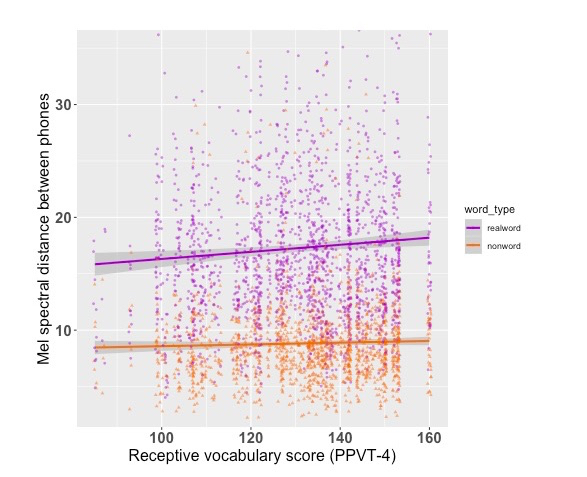
\includegraphics[scale=.7]{figures/figure_1.jpeg}
\caption{\label{fig:figure-1}CV coarticulation by receptive vocabulary score (PPVT-4)}
\end{figure}


\begin{table}[!htbp] \centering 
  \caption{Vocabulary and speech planning factors upon coarticulation} 
  \label{tab:model-1} 
\begin{tabular}{@{\extracolsep{5pt}}lc} 
\\[-1.8ex]\hline 
\hline \\[-1.8ex] 
 Intercept & 7.18$^{***}$ \\ 
  & (3.90, 10.47) \\ 
  & t = 4.29 \\ 
  & p = 0.0001 \\ 
  Word type [real word] & 5.41$^{**}$ \\ 
  & (2.08, 8.74) \\ 
  & t = 3.19 \\ 
  & p = 0.002 \\ 
  Receptive vocabulary score (PPVT-4) & 0.01 \\ 
  & ($-$0.01, 0.04) \\ 
  & t = 1.00 \\ 
  & p = 0.32 \\ 
  PPVT-4*Word type [real word] & 0.02$^{*}$ \\ 
  & (0.001, 0.05) \\ 
  & t = 2.08 \\ 
  & p = 0.04 \\ 
 \hline \\[-1.8ex] 
Observations & 3,449 \\ 
Log Likelihood & $-$10,756.98 \\ 
Akaike Inf. Crit. & 21,527.95 \\ 
Bayesian Inf. Crit. & 21,570.97 \\ 
\hline 
\hline \\[-1.8ex] 
\textit{Note:}  & \multicolumn{1}{r}{$^{*}$p$<$0.05; $^{**}$p$<$0.01; $^{***}$p$<$0.001} \\ 
\end{tabular} 
\end{table} 


\subsection{Spoken language experience and coarticulation}

After evaluating the roles of speech planning and vocabulary size for coarticulation, we turned to how the language environment may predict the children’s speech patterns and, more specifically, how the language environment could interact with speech planning and vocabulary. We predicted that the frequency of children’s vocalizations, quantified in daylong audio recordings, would mediate their coarticulation patterns: children who vocalize more often in daylong recordings will coarticulate less within CV sequences. 

To evaluate this hypothesis, an additional mixed effects linear regression model was fit to predict the Mel spectral distance between phones in each CV sequence. As before, a larger spectral distance indicates less gestural overlap---less coarticulation---between the segments.

To address the role of the environment on coarticulation, we included measures of the children’s daily language experiences from the 80 of the 103 children (77.7\%) who completed a daylong audio recording that was at least 9 hours long. The baseline model included the random effects of Word and Participant. We then repeated the forward model fitting procedure as before with the following parameters added: Phonotactic Transitional Probability, Second Syllable Frequency, Word Type, Late Talker, Maternal Education Level, Gender, Receptive Vocabulary Size (PPVT-4 growth scale value), Expressive Vocabulary Size (EVT-2 growth scale value), and Child Vocalization Count (the average number of hourly child vocalizations from the daylong recording). Predictors that did not improve model fit were removed from the analysis. 

Neither Phonotactic Transitional Probability nor Second Syllable Frequency improved upon a baseline model fit with just the random effects. The effect of Word Type was again significant even after fitting a model with Phonotactic Transitional Probability and another with Second Syllable Frequency. Thus, we again concluded that in this subset of 80 children who completed the daylong recordings, the effect of Word Type was independent of Second Syllable Frequency and Phonotactic Transitional Probability. We likewise did not find significant model improvements after adding Maternal Education Level, Gender, or Late Talker so we removed those factors from the model. 

Table \ref{tab:model-2} shows the final model fit: a significant main effect of Word Type, with a real word reference level again indicating that children coarticulated less in real words than nonwords (β=7.78, t=9.69 p<.001). Child Vocalization Count was also significant, indicating that children who tended to vocalize more throughout the daylong recording coarticulated less within CV sequences (β=.004, t=2.09, p=0.04), whether the sequences were embedded in nonwords or real words (Figure \ref{fig:figure-2}).\footnote{The vocabulary parameters were added to models without the Child Vocalization Count parameter to be sure that the absence of a vocabulary effect was not due to the presence of Child Vocalization Count.} This result provides some support for a ``practice effect'' for children’s coarticulation patterns.

The interaction of Word Type and Vocabulary Size (Expressive or Receptive) was not significant in this model fit to a subset of the children (N=80). Neither Expressive Vocabulary Size nor Receptive Vocabulary Size significantly improved upon a model with the effect of Word Type, though the improvement approached significance (improvement for model containing Expressive Vocabulary Size: X\textsubscript{2}=4.53, df=1, p=.10; Receptive Vocabulary Size: X\textsubscript{2}=4.37, df=1, p=.11). Thus, we did not replicate our findings on coarticulation and vocabulary size in this subset of 80 children.\footnote{Note that Child Vocalization Count and Receptive Vocabulary Size are not significantly correlated (r=.02, t=.16, p=.88). Nor are Child Vocalization Count and Expressive Vocabulary Size Pearson: r=-0.05, t=-0.47, p=.64. This lack of correlation between these variables indicates that children’s language skills and vocabulary sizes do not simply increase as they talk/vocalize more frequently.} 

We did want to explore the trends between vocabulary, child vocalizations, and coarticulation, however. Based on their receptive vocabulary scores, we performed a median split on the 80 children who had completed a daylong recording, dividing them into a smaller vocabulary group (n=42) and a larger vocabulary group (n=38). Dividing the children into these groups allowed us to see that the effect of Child Vocalization Count appears to be especially prominent for the children in the smaller vocabulary group (right panel of Figure \ref{fig:figure-2}). For the children with larger vocabularies, Child Vocalization Count does not appear to be strongly correlated in real words, only nonwords. However, these are simply trends in the data: a three-way interaction of Child Vocalization Count, Word Type, and Receptive Vocabulary did not approach significance.


\begin{figure}[H]
\centering
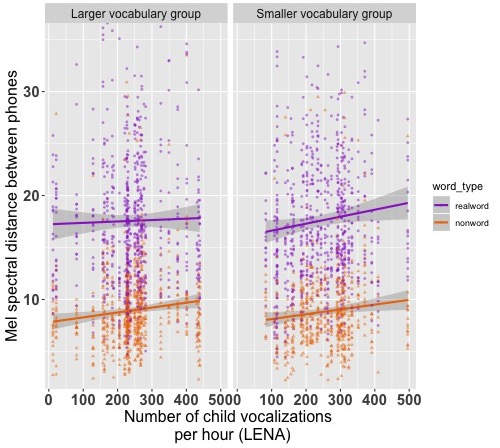
\includegraphics[scale=.7]{figures/figure_2.jpeg}
\caption{\label{fig:figure-2}Child vocalization count by Mel spectral distance between CV phones with a median split by receptive vocabulary size (PPVT-4). Child vocalization count was more predictive than receptive vocabulary size}
\end{figure}

\begin{table}[!htbp] \centering 
  \caption{Environmental and speech planning factors upon coarticulation} 
  \label{tab:model-2} 
\begin{tabular}{@{\extracolsep{5pt}}lc} 
\\[-1.8ex]\hline 
\hline \\[-1.8ex] 
 Intercept & 8.70$^{***}$ \\ 
  & (7.00, 10.40) \\ 
  & t = 10.04 \\ 
  & p = 0.00 \\ 
  Hourly child vocalization count & 0.004$^{*}$ \\ 
  & (0.0003, 0.01) \\ 
  & t = 2.09 \\ 
  & p = 0.04 \\ 
  Word type [real word] & 7.78$^{***}$ \\ 
  & (6.20, 9.35) \\ 
  & t = 9.69 \\ 
  & p = 0.00 \\ 
 \hline \\[-1.8ex] 
Observations & 2,781 \\ 
Log Likelihood & $-$8,701.94 \\ 
Akaike Inf. Crit. & 17,415.88 \\ 
Bayesian Inf. Crit. & 17,451.46 \\ 
\hline 
\hline \\[-1.8ex] 
\textit{Note:}  & \multicolumn{1}{r}{$^{*}$p$<$0.05; $^{**}$p$<$0.01; $^{***}$p$<$0.001} \\ 
\end{tabular} 
\end{table} 


\subsection{Language input and coarticulation}

Although we found that children who vocalized more in the daylong recordings coarticulated less within the CV sequences, these results could also be explained by parent-child engagement. Specifically, children’s vocalization quantity could be contingent upon adult language input. In our sample, we did find that the average number of hourly child vocalizations was positively correlated with the average number of hourly adult words (r=.44, t=4.35, p<.001; Figure \ref{fig:figure-3}). This led us to hypothesize that the quantity of adult speech in the child’s environment could predict the child’s coarticulation patterns, potentially having a stronger role than the child’s own productions. 


\begin{figure}[H]
\centering
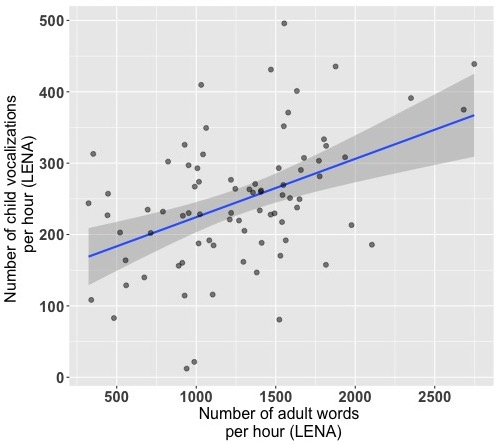
\includegraphics[scale=.8]{figures/figure_3.jpeg}
\caption{\label{fig:figure-3}Relationship between adult word count and child vocalization count}
\end{figure}

We tested this exploratory hypothesis in the same model of the 80 children who completed a daylong recording. Now instead of adding Child Vocalization Count, we instead added Adult Word Count, or the average number of words spoken by adults per hour in the daylong recording. Adult Word Count did not improve model fit, either with a model that included Child Vocalization Count (X\textsubscript{2}=.91, df=1, p=.34) or one that did not (X\textsubscript{2}=.006, df=1, p=.94). Therefore, we can confidently conclude that Adult Word Count does not directly predict children’s coarticulation within the CV sequences.

While we did not find a direct effect of Adult Word Count, the relationship between Adult Word Count and Child Vocalization Count, and in turn the relationship between Child Vocalization Count and degree of coarticulation, suggests an indirect role of Adult Word Count on children’s coarticulation: more adult words spoken in the environment leads to a greater number of child vocalizations, which, in turn, predicts the degree of children’s coarticulation. This relationship between the quantity of ambient adult language and coarticulation is indirect: Adult Word Count is not related to the children’s coarticulatory outcomes without factoring in Child Vocalization Count.  

\section{Discussion}

\subsection{Coarticulation in real words and nonwords}

Previous work has primarily attributed young children’s propensity to coarticulate to two factors: children’s immature, developing speech motor control \cite{barbierWhatAnticipatoryCoarticulation2020,rubertusDevelopmentGesturalOrganization2018,zharkovaDynamicsVoicelessSibilant2018} and the size of their representational units \cite{nittrouerEmergencePhoneticSegments1989,nittrouerHowChildrenLearn1996,noiraySpokenLanguageDevelopment2019,zharkovaCoarticulationIndicatorSpeech2011}. This study evaluated how several factors---speech planning, vocabulary size, and the language environment---predict coarticulation in a large cohort of four-year-old children. Crucially, each of these factors develops relatively independently of speech motor control. Thus, evaluating the relationships between the factors and the degree of children’s coarticulation allows us to determine some additional, underlying causes of coarticulation, beyond children’s developing motor control abilities. In the following sections, we discuss our findings concerning each of the three factors and their relationship with four-year-old children’s coarticulation patterns. 

To evaluate the role of speech planning for children’s coarticulation, the degree of the children’s coarticulation was measured in two environments: real words and corresponding nonwords (e.g. [su] in \textit{suitcase} and \textit{sudras}). We predicted that children would coarticulate less between CV sequences embedded in real words than nonwords because children have more experience with the real words. 

Our analyses supported this prediction. Children coarticulated significantly less in real words than nonwords. This conclusion may appear counterintuitive to some audiences: how could children coarticulate more in words that they have not previously practiced? In adults coarticulation is usually planned \cite{whalenCoarticulationLargelyPlanned1990} and reflects an equilibrium between speaker efficiency and listener comprehension \cite{bradlowConfluentTalkerListeneroriented2002}. However, it is important to remember that children do not coarticulate for the same reasons as adults. As we have outlined in this paper, child coarticulation is generally attributed to a lack of fine motor control and entrenched articulatory schema that may be required to differentiate between adjacent phones during speech \cite{goffmanRelationsSegmentalMotor2007,greenPhysiologicDevelopmentSpeech2000,mcallisterbyunMotorInfluencesGrammar2016} or phonological reorganization \cite{nittrouerEmergencePhoneticSegments1989,nittrouerHowChildrenLearn1996,noiraySpokenLanguageDevelopment2019,redfordGrammaticalWordProduction2018,zharkovaCoarticulationIndicatorSpeech2011}. Consequently, children should be expected to coarticulate less in those contexts where they have more experience.

Why do children coarticulate less in real words than the matched nonwords? One explanation could be that the task demands of nonword repetition differ from those of real word repetition. For example, while the CV sequence was matched across each real word and nonword pair, nonword production requires repetition without any phonetic, lexical, or semantic support. Speakers must encode and produce a novel combination of syllables without reinforcement. In real word repetition, on the other hand, speakers must encode a semantic and phono-lexical representation and then execute the associated articulatory schema. Nonword repetition is also often considered a proxy for phonological representations in working memory (e.g., \citeNP{edwardsNonwordRepetitionsChildren1998,gathercoleNonwordRepetitionWord2006}): children with larger vocabularies perform better on the task \cite{edwardsInteractionVocabularySize2004,munsonRelationshipsNonwordRepetition2005} and speakers of all ages perform worse on longer, multisyllabic words \cite{byrdNonwordRepetitionPhoneme2012}.\footnote{Nonword repetition is a proxy for phonological working memory, but there are myriad factors, including those pertaining to the stimuli like phoneme frequency and sub-syllabic frequency, that predict task performance (see \citeauthor{szewczykNonwordRepetitionDepends2018} (2018) for comprehensive overview).} The task demands that nonword repetition placed on the children in this study could then have affected the children’s coarticulation by not permitting the same degree of planning permitted for real word repetition. This, in addition to the fact that children cannot rely upon established motor schemata to articulate the nonwords, may explain the coarticulation differences between the two tasks. 

Another possible explanation for the different coarticulation patterns between nonwords and real words is that the production differences reflect children’s phonological reorganization. Less coarticulation in real words could reflect the emergent abstraction of phonological units \cite{mcallisterbyunMotorInfluencesGrammar2016,nittrouerEmergencePhoneticSegments1989,nittrouerHowChildrenLearn1996,zharkovaCoarticulationIndicatorSpeech2011}, specifically the reorganization of phonological representations from larger sub-lexical units like syllables and feet into smaller, phoneme-sized ones. According to theories that ascribe the development of phonological categories to generalizations children make over their vocabularies \cite{beckmanGeneralizingLexiconsPredict2010,metsalaSpokenVocabularyGrowth1998,sosaLexicalPhonologicalEffects2012,stoel-gammonRelationshipsLexicalPhonological2011}, we might expect children to have more abstract speech segments in real words---which the children have heard, produced, and practiced before---than nonwords. This phonological abstraction could then play out in the children’s speech production: children coarticulate less in real words than corresponding nonwords. 

In the following section we attempt to disentangle these two explanations by exploring the interactions between coarticulation in the repetition tasks and the children’s individual differences in vocabulary size and vocalization frequency. 

\subsection{Language experience and coarticulation}

\subsubsection{The role of vocabulary size on coarticulation}

Our second hypothesis concerned the role of vocabulary size on child coarticulation patterns in the real words and nonwords. Using our full sample size of 103 children, we found that children with larger receptive vocabularies coarticulated less between the segments in CV sequences.\footnote{Receptive vocabulary size was marginally more predictive of coarticulation degree than expressive vocabulary size. The difference between these models was marginal, and expressive and receptive vocabulary scores are correlated, so we do not make strong claims concerning the role of receptive versus expressive vocabulary for coarticulation patterns. Both estimates of vocabulary size appear to predict coarticulation to a similar degree.} The significant interaction of receptive vocabulary size and word type demonstrated that children with larger receptive vocabularies showed the largest discrepancy in coarticulation patterns by word type. 

The finding that children with larger vocabularies coarticulate less is unsurprising. In the one study that has previously evaluated a relationship between vocabulary size and degree of coarticulation in young children, the authors found that children aged 4;0-7;0 with larger expressive vocabularies showed less anticipatory coarticulation in [stop]-V sequences \cite{noiraySpokenLanguageDevelopment2019}. \citeauthor{noiraySpokenLanguageDevelopment2019} (2019) attribute this relationship between vocabulary size and coarticulation to the primacy of the lexicon for phonetic and phonological development, and production accuracy in particular \cite{beckmanGeneralizingLexiconsPredict2010,edwardsInteractionVocabularySize2004,metsalaYoungChildrenPhonological1999,metsalaSpokenVocabularyGrowth1998,storkelInfluencePartwordPhonotactic2011,storkelLexiconPhonologyInteractions2002}. Children with larger vocabularies have been shown to perform better on nonword repetition accuracy (3;2-8;10: \citeNP{edwardsInteractionVocabularySize2004}; 3;0-6;0: \citeNP{munsonRelationshipsNonwordRepetition2005}) and novel word learning (2;11-6;0: \citeNP{storkelInfluencePartwordPhonotactic2011}). The finding that children with larger vocabularies also coarticulate less is consistent with these previous results. 

Still, the relationship between receptive vocabulary size and coarticulation observed here is not as robust as the relationship between vocabulary size and the other outcome measures (repetition accuracy, novel word learning) evaluated elsewhere \cite{edwardsInteractionVocabularySize2004,metsalaYoungChildrenPhonological1999,storkelInfluencePartwordPhonotactic2011}. This could be because there are myriad other factors, beyond vocabulary size, that predict children’s spoken phonetic outcomes and coarticulation in particular. 

Throughout this work, we have entertained two explanations for children’s coarticulation patterns: speech motor control and phonological reorganization. The finding that children with larger vocabularies coarticulate less supports the idea that coarticulation reflects phonological reorganization from larger sub-lexical units into phonemes. This is because previous work has concluded that children with larger vocabularies have more segmental phonological representations (e.g. \citeNP{metsalaSpokenVocabularyGrowth1998}). However, the weaker relationship between coarticulation and vocabulary size, compared to previous work evaluating the relationship between word learning or repetition accuracy and vocabulary size, suggests that there is also a strong role of another factor for children’s coarticulation---fine motor control---that may not explain as much variability in novel word learning or nonword repetition accuracy. The result is that vocabulary size does predict the degree of children’s coarticulation, but the effect may be weaker because fine motor control exerts a strong influence on the degree of coarticulation \cite{barbierWhatAnticipatoryCoarticulation2020}.

Another interesting conclusion from the vocabulary results was that children with larger vocabularies showed the largest difference in coarticulation patterns by word type. Specifically, the effect of vocabulary size on coarticulation was strongest for real words. In previous work, any difference between nonword repetition accuracy by phonotactic frequency \cite{edwardsInteractionVocabularySize2004} or lexical status \cite{cychoszLexicalAdvantageFouryearold2020} was less apparent in the children with larger vocabularies. Those findings suggested that the children with larger vocabularies were able to generalize their experience with high-probability sequences or real words to novel environments such as nonwords. We propose that children with larger vocabularies have more practiced routines for real words than nonwords---and that they have much more practiced routines for real words than the children with smaller vocabularies. As a result, children with larger vocabularies show the greatest disparity in coarticulation by word type. 

\subsubsection{The role of production practice on coarticulation}

The final potential predictor of children’s coarticulation that we evaluated in this study was the language environment, specifically the frequency of children’s vocalizations. This was examined in the subset of children who completed a daylong audio recording (80/103 or 77.7\%) and we found that children who vocalized more during the daylong recording coarticulated less, both in real words and nonwords. Previous research has documented a production advantage or ``practice effect'' for a variety of speech and language tasks (\citeNP{depaolisProductionPatternsInfluence2011,depaolisInfluenceBabblingPatterns2013,ichtProductionEffectMemory2015,keren-portnoyRoleVocalPractice2010,majoranoRelationshipInfantsProduction2014} cf. \citeNP{zamunerReverseProductionEffect2018}) whereby children who practice more spoken language, or articulate words during word learning, could learn to encode articulatory movements with their acoustic representations. This, in turn, may further entrench phonological representations and may make the task of accessing a given word or phone easier, and smoother, for future productions. This study was the first to examine this practice effect in older children, aged 4;0, using naturalistic recordings of the children’s everyday environments and our results corroborate previous evidence in support of a practice effect for speech development.

It should be noted that our estimate of hourly child vocalizations was relatively coarse. While the child vocalization count estimator of the LENA speech parsing algorithm performs reliably well \cite{cristiaThoroughEvaluationLanguage2020} (better than other more language- and context-specific estimations from LENA), the algorithm does not distinguish between speech-like vocalizations and crying or laughing. Consequently, this study is an important first step in establishing the role of self-practice for children’s coarticulation and speech development. Future work now needs to evaluate children’s naturalistic speech productions in this age range in a more fine-grained manner to better understand what characteristics of children’s vocalizations predict their speech outcomes. For example, while we did not find that an estimate of receptive language experience, adult word count, directly predicted the degree of coarticulation, adult word count and child vocalization count were positively correlated. Thus, it could be that interactions with adult interlocutors in particular indirectly predict coarticulatory development. Delving deeper into the role of self-practice and the language learning environment is thus an important area for future research on phonetic development. 

\subsection{On data exclusion and daylong recordings}

As daylong recording methodologies increase in popularity in developmental language research, ethical issues surrounding participant exclusion will become more apparent \cite{casillasStepbystepGuideCollecting2019}. In this study, 22 families opted not to participate in the daylong recording portion of the study. We still included the word repetition and vocabulary data for these children rather than excluding them completely from the study. 

Daylong recordings require that children wear recorders over extended periods. Sound within an approximately five foot radius of the child is captured in the recording. Some families may, understandably, not be comfortable with this methodology. One solution for studies like ours that incorporate covariates derived from daylong recordings could be to exclude all children whose families opt out of the daylong recording. However, we do not encourage this option. The decision to contribute a daylong audio recording to a research study may depend on several external factors like socioeconomic status, race, and familial structure (i.e. single-parent households). For example, in a hypothetical example that relates to the current study, some caregivers may have unpredictable work schedules making it difficult to complete a 12 hour recording. Given these challenges, it would hardly be surprising if some individuals from under-served communities were more likely to opt out of daylong recording methodologies. In fact, in our sample, we found a different SES distribution in families who completed the daylong recording (92.59\% of mothers had more than a high school diploma) versus those who did not (86.36\% of mothers had more than a high school diploma).\footnote{ The SES breakdown of the two groups was as follows: for families who did complete a daylong recording n=1 did not have a high school diploma, n=1 had the equivalent of a high school diploma (e.g. GED), n=4 had a high school diploma, n=0 had <2 years of college, n=15 had 2+ years of college, n=27 had completed college, and n=33 had graduate degrees . For families who did not complete a daylong recording, n=1 did not have a high diploma, n=0 had the equivalent of a high school diploma, n=2 had a high school diploma, n=1 had <2 years of college, n=6 had 2+ years of college, n=6 had completed college, and n=6 had graduate degrees.} Thus, excluding all families who could not complete a daylong recording could inadvertently exclude some groups from representation in social science research. The exclusion of these families would not be random and could, inadvertently, serve to further bias language development findings for upper middle class North American children. 

\subsection{The status of children’s phonological representations}

An overarching goal of this study was to contribute to our understanding of children’s phonological representations, and to understand how those representations differ from adults’. By showing novel evidence for the roles of speech planning, vocabulary size, and the language environment on coarticulation, this study corroborates \citeauthor{noiraySpokenLanguageDevelopment2019} (2019) in suggesting that coarticulation is dually explained by speech motor control maturation and phonological reorganization. In particular, the predictive relationship of vocabulary size for coarticulation found in this study suggests that children with larger lexicons have more segmental phonological units. This supports phonological reorganization. 

The ramifications for the role of child vocalization frequency may be less straightforward because algorithmically-derived speech measures, such as LENA’s child vocalization count or adult word count, do not necessarily map onto linguistically-coded categories. Children who vocalized more often during the daylong recording may exhibit motor practice effects, resulting in more entrenched or even abstracted phonological categories. Of course children who vocalize more could also have greater motor control because they speak more frequently. The hourly child vocalization count derived from the LENA recordings was more predictive than vocabulary size (receptive or expressive) for coarticulation in the participants where we could test both vocabulary size and child vocalization count. Indeed, we did not even replicate the relationship between vocabulary size and degree of coarticulation in the subset of children who completed daylong audio recordings (the effect only approached significance and trended in the expected direction). On the basis of the comparison of these two factors, it appears that the frequency of speech practice is the strongest predictor of children’s coarticulation patterns. 

\section{Conclusion}

This study measured four-year-old children’s coarticulation between phones in CV sequences. Previous work on this topic has struggled to disentangle the roles of fine motor control and the potential role of children’s larger representational units for children’s coarticulation patterns. Three factors that develop relatively independently of fine motor control---speech planning, vocabulary size, and the language environment---were evaluated for their role on coarticulation. Children coarticulated less in real words than nonwords and children with larger vocabularies coarticulated less overall, and in real words in particular. Children who vocalized more throughout the day also coarticulated less. This daily practice effect was more predictive of coarticulatory outcomes than vocabulary size or the quantity of adult language in the ambient environment. The relatively larger effect of vocalization frequency measure over vocabulary size preliminarily suggests the primacy of fine motor control for coarticulation development. (Word count: 10793)

\section{Acknowledgements}

The authors wish to acknowledge the families who participated in this research. We also thank many members of the Learning to Talk Labs at the University of Wisconsin, Madison and the University of Minnesota, Twin Cities for assistance with data collection. Additional thanks to Rebecca Higgins at the University of Maryland, College Park for her assistance in data processing. This research was supported by the Raymond H. Stetson Scholarship in Phonetics and Speech Science (M.C.) and National Institute on Deafness and Other Communication Disorders Grant T32DC000046 (M.C.) and R0102932 (J.R.E., B.M., and Mary E. Beckman).   

\section{Declaration of interest}

The authors have no conflicts of interest to report. 



\bibliography{zotero_library}

\begin{figure}[H]
\centering
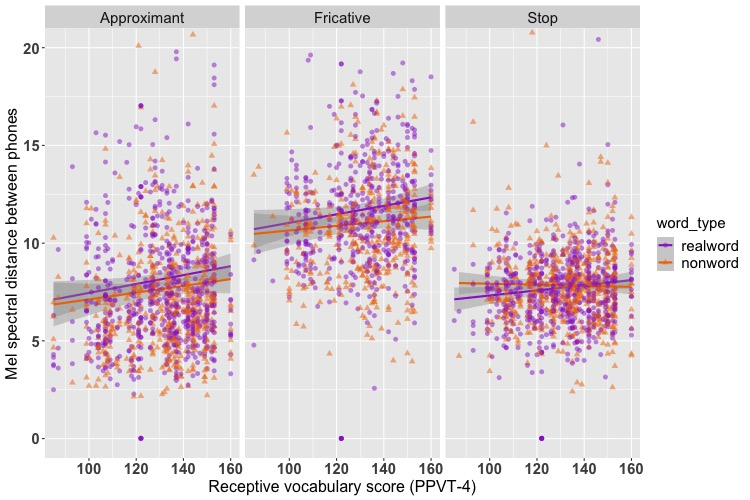
\includegraphics[scale=.7]{figures/figure_4.jpeg}
\caption{\label{fig:figure-4}CV coarticulation by receptive vocabulary size and consonant manner}
\end{figure}

\begin{figure}[H]
\centering
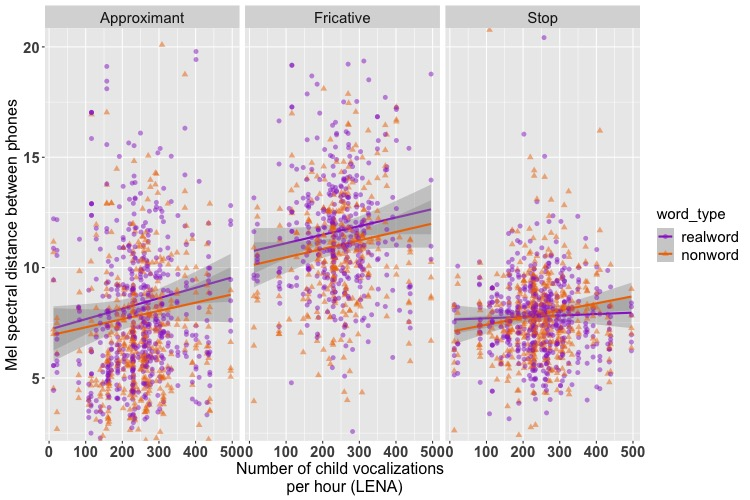
\includegraphics[scale=.7]{figures/figure_5.jpeg}
\caption{\label{fig:figure-5}CV coarticulation by number of child vocalizations and consonant manner}
\end{figure}

\end{document}